
General relativity describes how matter and energy curve the fabric of space and time.
Einstein first wrote down the theory more than a century ago, and it is still our most accurate theory of gravitational effects.
It makes accurate and counterintuitive predictions, which experiments have borne out.
This chapter surveys the basics of general relativity and some mathematical prerequisites.
We will then use this to derive the Tolman-Oppenheimer-Volkoff (TOV) equation, a differential equation used to model stars.
This chapter is based on~\autocite{carrollSpacetimeGeometryIntroduction2019,leeSmoothManifolds2012}.

\section{Differential geometry}

\begin{figure}[ht]
    \centering
    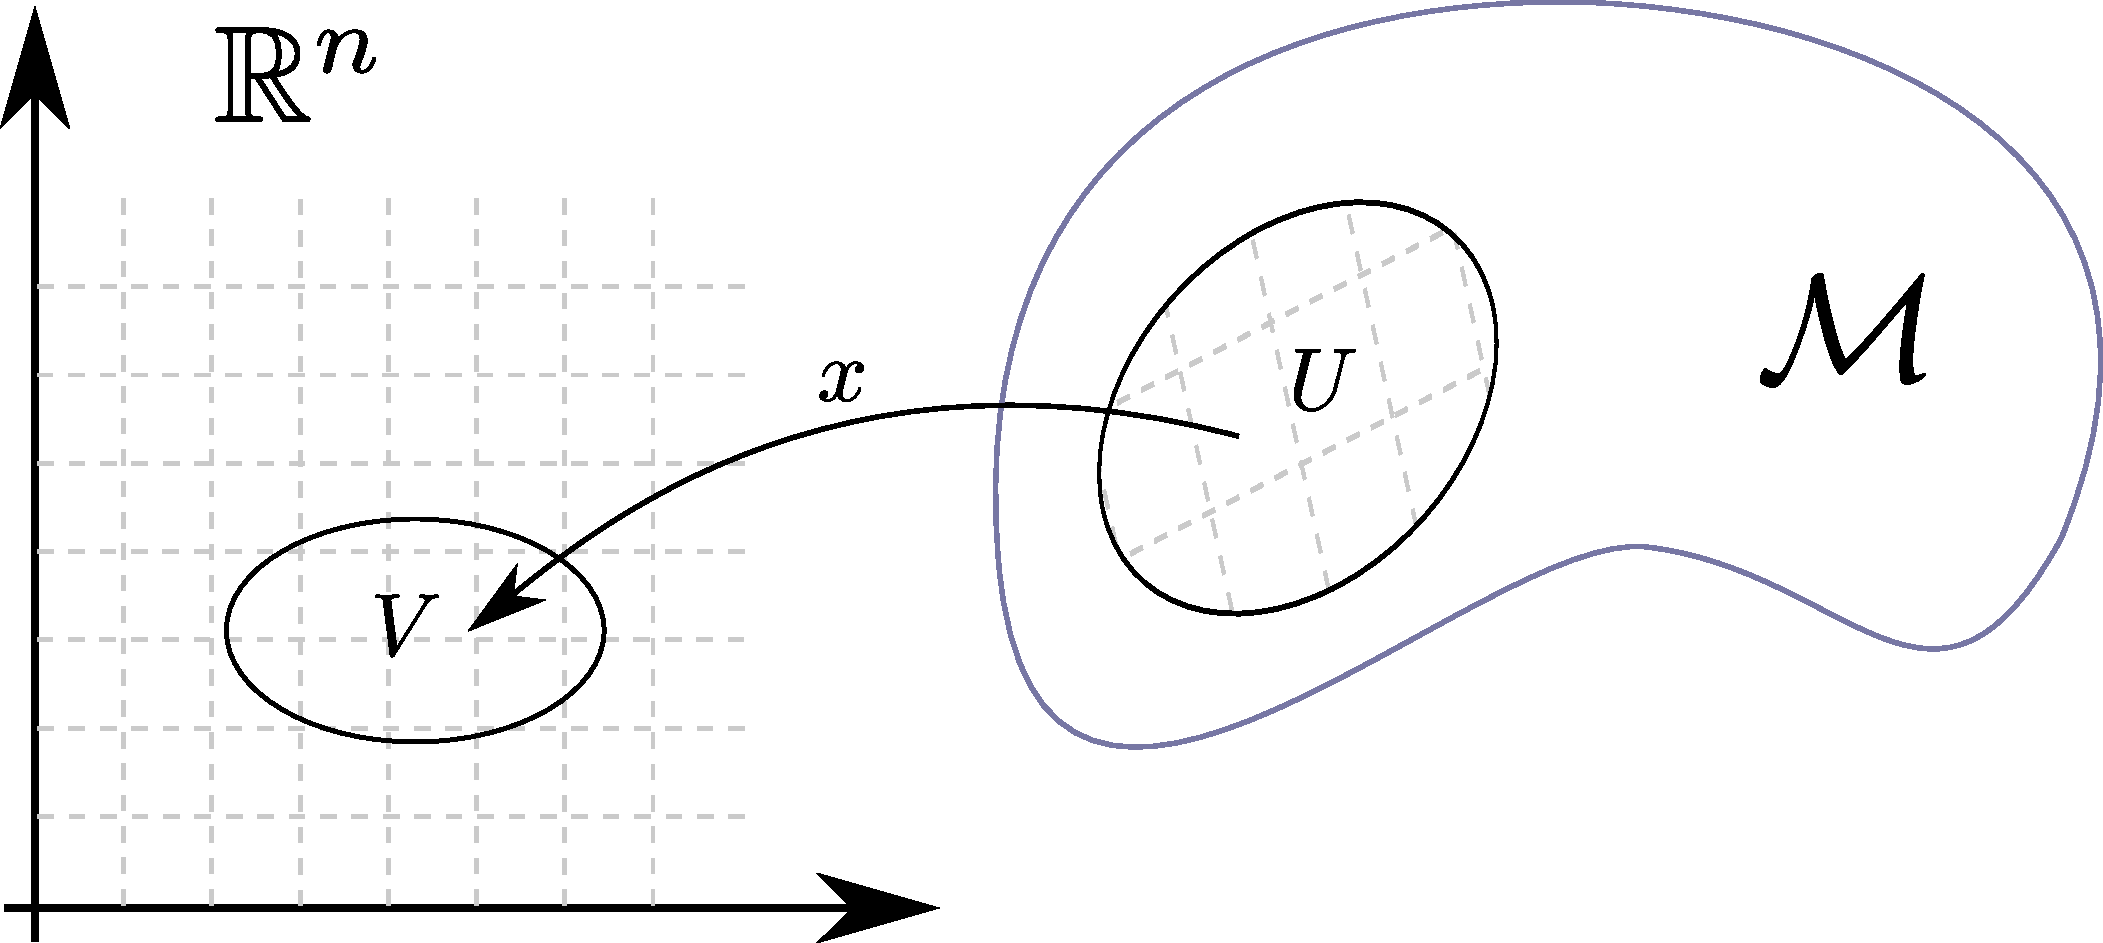
\includegraphics[width=0.6\textwidth]{figurer/coordinate_function.pdf}
    \label{coordinate function}
    \caption{(Kladd) The coordinate function $x$ maps a neighborhood $U$ in the manifold $\Em$ to a negiborhood $V$ in $\R^n$.}
\end{figure}


General relativity is formulated in the language of \emph{differential geometry}, which generalizes multivariable calculus to more general spaces than $\R^n$.
These spaces are \emph{smooth manifolds}.
A $n$-dimensional manifold, $\Em$, is a set of points, locally homeomorphic to $\R^n$.
That is, for all points $p \in \Em$, there exists a neighborhood $U$ around $p$, together with a corresponding set of continuous, bijective functions,
%
\begin{align}
    x: U \subseteq \Em & \longmapsto V \subseteq \R^n, \\
    p & \longmapsto x^\mu(p).
\end{align}
%
We call $x(p) = (x^0(p), \dots, x^{n- 1}(p)) = x^\mu(p)$ a coordinate function of $\Em$.
The inverse of $x$, $x^{-1}$, obeys $x^{-1}(x(p)) = p$, for all $p \in U$.
A smooth manifold is one in which the coordinate functions are infinitely differentiable.
Differentiability is defined by considering two different coordinate functions, $x$, and $x'$.
The corresponding domains $U$ and $U'$ may or may not overlap.
We then define the transition function, a function between subsets of $\R^n$ by mapping via $\Em$, as
%
\begin{align}
    f_{x'\rightarrow x} = x' \circ x^{-1} : \R^n \mapsto \R^n.
\end{align}
%
The map is illustrated in \autoref{fig: transition map}.
\footnote{To be rigorous, one has to restrict the domains and image of the coordinate function when combining them.}
A set of coordinate functions $\mathcal A = \{x_i\}$ whose domain cover $\Em$ is called an \emph{atlas} of $\Em$.
If the transition function between all pairings of coordinate functions in the atlas is smooth---that is, infinitely differentiable---we call the atlas smooth.
We then define a smooth manifold as the topological manifold $\Em$ together with a \emph{maximal} smooth atlas $\mathcal A$.
A smooth atlas is maximal if no coordinate function can be added while the atlas remains smooth.\footnote{%
    The maximal condition is to ensure that two equivalent atlases correspond to the same differentiable manifold. A single manifold can be combined with different maximal atlases, also called differentiable structures. 
    }
%
\begin{figure}
    \centering
    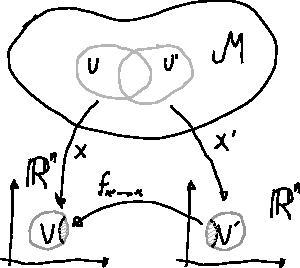
\includegraphics[width=0.5\textwidth]{figurer/transition_map_kladsvg.pdf}
    \caption{
        (Kladd) The transition map $f_{x'\rightarrow x}$ between two coordinate functions, $x$ and $x'$, maps between the images of these function, via the manifold $\Em$. The function's domain and image are restricted to a (possibly empty) subset of the images of $x$ and $x'$. This is illustrated by the shaded regions in $V$ and $V'$. 
        }
    \label{fig: transition map}
\end{figure}

Consider two $m$- and $n$-dimensional smooth manifolds $\Em$ and $\mathcal N$.
Let $x$ denoted the coordinates on $\Em$, while $y$ denotes the coordinates on $\mathcal N$.
We can define smooth functions between these manifolds similarly to how we define smooth coordinates.
Consider the function
%
\begin{equation}
    F: \Em \longmapsto \mathcal N.
\end{equation}
%
It is said to be smooth if, for all points $p \in M$, there is a set of local coordinates $x$ around $p$ and $y$ around $F(p)$ such that the map $\tilde F = y \circ F \circ x^{-1}$ is smooth.
This map is defined by the diagram
%
\begin{equation}
    % https://tikzcd.yichuanshen.de/#N4Igdg9gJgpgziAXAbVABwnAlgFyxMJZABgBoBGAXVJADcBDAGwFcYkQAdDgW3pwAsARoIAEAJQB63EAF9S6TLnyEUZYtTpNW7LrwEBjJiICys+SAzY8BIuVLqaDFm0SceffocYiAcmYVWyrYUGk7arroewuIShDIaMFAA5vBEoABmAE4Q0oh2IDgQSGQgjPSCMIwACorWKqUw6TggjlouIAAe-iBZOUj5hUgATK3O7OndvbkjBUWIAMyj4SAAnpPZuSWDC0vtSbKUMkA
\begin{tikzcd}
    \mathcal M \arrow[d, "x"] \arrow[r, "F"] & \mathcal N \arrow[d, "y"] \\
    \mathbb R^m \arrow[r, "\tilde F"]               & \mathbb R^n              
    \end{tikzcd}
    %
\end{equation}
%
%
We will not be careful with the distinction between $F$, the function between the abstract manifolds, and $\tilde F$, the function of their coordinates, but rather denote both by $F(x)$.
We may take the partial derivative of such a function with respect to the coordinates $x$, $\diffp{F}/{x^\mu}$.
However, this is obviously dependent on our choice of coordinates, as a set of local coordinates can always be scaled.
Any physical theory must be independent of our choice of coordinates, so our next task is to define the properties of a smooth manifold in a coordinate independent way.

\subsection*{Vectors and tensors}

A curve $\gamma$ through $\Em$ is a function from $\R$ to $\Em$,
%
\begin{align}
    \gamma : \R &\longmapsto \Em \\
    \lambda & \longmapsto \gamma(\lambda).
\end{align}
%
Such curves are often denoted only by their coordinates and the parameter $\lambda$, $x^\mu(\lambda) = (x^\mu \circ \gamma)(\lambda)$.
With this curve, we can take the directional derivative of a real-valued function on the manifold, $f: \Em \mapsto \R$.
Assume $\gamma(\lambda = 0) = p$.
As we are always taking the derivative of functions between $\R^n$, for different $n$, we can use the chain rule.
The directional derivative of $f$ at $p$, given by this curve $\gamma$, is then
%
\begin{equation}
    \diff{}{\lambda} f(x(\lambda)) \bigg |_p = \diff{x^\mu}{\lambda} \bigg |_{\lambda = 0}  \diffp{}{x^\mu} f(x) \bigg |_p.
\end{equation}
%
The set of all such directional derivatives, $\diff{}/{\lambda}$ at $p$, form a vector space, $T_p \Em$, called the \emph{tangent space}.
The tangent space is illustrated in \autoref{fig: tangent space}.
The coordinates $x^\mu$ induce a basis of this vector space,
\todo{Find the best notation here}
%
\begin{equation}
    e_\mu = \diffp{}{x^\mu} \Big|_p = \partial_\mu|_p, \quad \mu \in \{0, ... n-1\},
\end{equation}
%
so any element $v \in T_p \Em$ can be written
%
\begin{equation}
    v = v^\mu \partial_\mu |_p = \diff{x^\mu}{\lambda}\Big |_{\lambda = 0} \diffp{}{x^\mu}\Big |_p.
\end{equation}
%
Here, $\lambda$ is the parameter of the curve corresponding to the directional derivative $v$.\footnote{%
There is not only one curve corresponding to any directional derivative but rather an equivalence class.
}
We assume $\lambda = 0$ corresponds to $p$.
The evaluation at $\lambda = 0$ and $p$ will often be implicit for ease of notation.
This directional derivative acts on functions $f : \Em \mapsto \R$ as
%
\begin{equation}
    v(f) = v^\mu \partial_\mu f.
\end{equation}
%

\begin{figure}[ht]
    \centering
    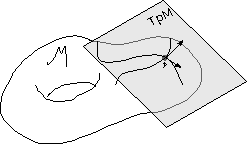
\includegraphics[width=0.5\textwidth]{figurer/tangent space.pdf} 
    \caption{
        (Kladd) The tangent space $T_p \Em$, the shaded rectangle, is the sett of all directional derivatives at $p\in \Em$. A directional derivative is defined in terms of a curve that passes through $p$.
        } 
    \label{fig: tangent space}
\end{figure}



A map $F$ between two manifolds $\Em$ and $\mathcal N$ also induces a map between the tangent spaces of these manifolds.
This is the \emph{differential} of $F$ at $p$, 
%
\begin{align}
    \dd F_p: T_p \Em & \longmapsto T_p \mathcal N, \\
    v & \longmapsto \dd F_p (v). 
\end{align}
%
As $\dd F_p(v)$ is an element of $T_p \mathcal N$,   directional derivative on $\mathcal N$, defined as
%
\begin{equation}
    \dd F_p(v) (g) = v(g \circ F),
\end{equation}
%
for functions $g : \mathcal N \mapsto \R$.
It thus acts on functions on $\mathcal N$ by ``extending'' the derivative $v$.
This is a linear map between vector spaces and may be written in component form by considering the differentials of the coordinate functions.
Denote the coordinates of $\mathcal N$ by $y^\mu$, and $y^\mu \circ F = F^\mu$.
Then,
%
\begin{equation}
    \dd F_p (\partial_\mu) (g) = \partial_\mu (g \circ F) |_p 
    = \diffp{F^\nu}{x^\mu}\Big |_p \diffp{g}{y^\nu} \Big  |_{F(p)},
\end{equation}
%
or more suggestively
%
\begin{equation}
    \dd F \left( \diffp{}{x^\mu} \right) = \diffp{F^\nu}{x^\mu} \diffp{}{y_\nu}.
\end{equation}
%
The differential is thus a generalization of the Jacobian of a function.
In the case of a real valued function, $f: \Em \mapsto \R$, and $g : \R \mapsto \R$, we get
%
\begin{equation}
    \dd f (v) (g) 
    = v(g \circ f) 
    = (v^\mu \partial_\mu f) \, \diff{g}{y}.
\end{equation}
%
$\dd f$ is thus a map from $T_p \Em$ to $\_{f(p)}\R$, which is isomorphic to $\R$, i.e.,
it is a map from vectors $v$ to real numbers,
%
\begin{equation}
    \dd f(v) = \dd f(v)(y) = v^\mu \partial_\mu f.
\end{equation}
%
The set of all linear maps from a vector space $V$ to the real numbers is called the \emph{dual space} of $V$, and is denoted $V^*$.
This is a new vector space with the same dimensionality of $V$.
We denote the dual of $T_p \Em$ as $T_p^* \Em$.
We can regard each of the coordinate functions as real-valued functions, with a corresponding differential.
This differential obeys
%
\begin{equation}
    \dd x^\mu (\partial_\nu) = \diffp{x^\mu}{x_\nu} = \delta^\mu_\nu.
\end{equation}
%
The differentials of the coordinate functions thus form a basis for $T^*_p \Em$, called the dual basis.
Using this, we can assume $\dd f = \omega_\mu \dd x^\nu$ for some components $\omega_\mu$, and find that $\omega_\mu = \partial_\mu f$.
Or, in other words, we recover a rigorous justification for the classical expression 
%
\begin{equation}
    \dd f = \diffp{f}{x^\mu} \dd x^\mu,
\end{equation}
however we now interpret it as a covector-field instead of an ``infinitesimal displacement''.

Linear map from vectors to real numbers is generalized by \emph{tensors}.
Given a vector space $V$, a general $(n, m)$ tensor $T$ is a multilinear map, which associates $n$ elements from $V$ and $m$ from its dual $V^*$ to the real numbers, i.e.,
%
\begin{align}
    T: V \times V \times \dots\times V^* \times \dots &\longmapsto \R, \\
    (v, u\dots; \omega, \dots) & \longmapsto T(v, u, \dots; \omega, \dots).
\end{align}
%
Multilinear means that $T$ is linear in each argument.
The set of all such maps is the tensor product space $V\otimes V \otimes \dots \otimes V^* \otimes \dots$, a $\dim(V)^{n+m}$-dimensional vector space.
If $\{e_\mu\}$ and $\{e^\mu\}$ are the basis for $V$ and $V^*$, then we can write the basis of this of the tensor product space as $ \{e_{\mu} \otimes\dots \otimes e^{\nu} \otimes \dots \}$.
The tensor can thus be written
%
\begin{equation}
    T = T^{\mu \nu\dots}{}_{\rho\dots} \, e_{\mu}\otimes e_\nu \otimes \dots e^\rho\otimes\dots, 
\end{equation}
% 
where
%
\begin{equation}
    T^{\mu \nu\dots}{}_{\rho\dots} = T(e^\mu e^\nu, \dots; e_\rho, \dots).
\end{equation}


\subsection*{Geometries and the metric}

The metric is a symmetric, non-degenerate $(0, 2)$ tensor
%
\begin{equation}
    \dd s^2 = g_{\mu \nu} \, \dd x^\mu \otimes \dd x^\nu.
\end{equation}
%
It defines the geometry of the manifold $\Em$, and is the main object of study in general relativity.
As it is invertible, we can define $g^{\mu \nu} = (g^{-1})_{\mu \nu}$, which is the components of a $(2, 0)$ tensor.
We use this to raise and lower indices, as is done with the Minkowski metric $\eta_{\mu \nu}$ in special relativity.

Up until now, we have only considered the tangent space $T_p \Em$ at a point $p$.
We are, however, more interested in fields of vectors, covectors, or tensors.
For each point $p \in \Em$, a tensor field $T$ ``picks out'' a tensor $T(p)$ from each tensor product space corresponding to the tangent space at $p$, $T_p \Em$.
We will use a vector field to illustrate.
This vector field can be written as
%
\begin{equation}
    v(p) = v^\mu(p) \partial_\mu |_p. 
\end{equation}
%
We will mostly be working with the components $v^\mu$, which are functions of $\Em$.
For ease of notation, we write the vector as a function of the coordinates $x$.
The vector field $v(x)$ is unchanged by a coordinate-transformation $x^\mu \rightarrow {x'}^\mu$; the coordinate is only for our convenience.
However, with a new set of coordinates, we get a new set of basis vectors, $\partial'_\mu$:
%
\begin{equation}
    v = v^\mu \partial_\mu = v^\mu \diffp{x'^\nu}{x^\mu} \partial'_\nu
    = v'^\mu \partial_\mu',
\end{equation}
%
This gives us the transformation rules for the components of vectors,
%
\begin{equation}
    v'^\mu = \diffp{x'^\mu}{x^\nu} v^\nu.
\end{equation}
%
Tangent vectors are also called \emph{contravariant} vectors, as their components transform contra to basis vectors.
For covectors, it is
%
\begin{equation}
    \omega'_\mu = \diffp{x^\nu}{x'^\mu} \omega_\nu,
\end{equation}
%
which is why covectors also are called \emph{covariant} vectors.

The gradient of a scalar function $f$, $\dd f = \partial_\mu f \dd x^\mu$, is a coordinate-independent derivative, as $\partial_\mu f$ follows the transformation law for covectors.
We define the covariant derivative, $\nabla$, as a map from $(n, m)$ tensor fields to $(n, m+1)$ tensor fields.
When considering a scalar as a $(0, 0)$ tensor, we see that this generalizes the scalar derivative.
Of the covariant derivative, we assume
%
\begin{itemize}
    \item Linearity: $\nabla (T + S) = \nabla T + \nabla S$.
    \item The product rule: $\nabla (T \otimes S) = (\nabla T)\otimes S + T \otimes (\nabla S)$.
    \item Reduces to partial derivative for scalars: $\nabla_\mu f = \partial_\mu f$.
    \item Kronecker delta gives zero: $\nabla_\mu \delta^\rho_\nu = 0$.
\end{itemize}
%
With this, we can, in general, write the covariant derivative as~\autocite{carrollSpacetimeGeometryIntroduction2019}
%
\begin{align}
    \nabla_\mu v^\nu &= \partial_\mu v^\mu + \Gamma^\mu_{\nu \rho} v^\rho, \\
    \nabla_\mu \omega_\nu &= \partial_\mu \omega_\nu - \Gamma^\rho_{\mu \nu} \omega_\rho,
\end{align}
%
for vectors and covectors.
$\Gamma^{\mu}_{\nu \rho}$ are called \emph{Christoffel symbols}.
The generalization for higher-order tensors is straightforward, 
%
\begin{equation}
    \nabla_\mu T^{\nu\dots}{}_{\rho\dots}
    =
    \partial_\mu T^{\nu\dots}{}_{\rho\dots}
    + \Gamma^\mu_{\nu \lambda} T^{\lambda\dots}{}_{\rho\dots} +\dots
    - \Gamma^\lambda_{\mu \rho} T^{\mu\dots}{}_{\lambda\dots} -\dots.
\end{equation}
%
This is still not enough to uniquely determine the covariant derivative.
We will furthermore assume $\Gamma^{\lambda}_{\mu \nu} = \Gamma^{\lambda}_{\nu \mu}$ and $\nabla_\mu g_{\nu \rho} = 0$.
With these, we can find an explicit formula of the Christoffel symbols in terms of the metric,
%
\begin{equation}
    \label{christoffel symbols from metric}
    \Gamma^\rho_{\mu \nu} = \frac{1}{2} g^{\rho \sigma} (\partial_\mu g_{\nu \sigma} - \partial_\sigma g_{\mu \nu} + \partial_{\nu}g_{\sigma \mu}).
\end{equation}
%

The curvature of a manifold $\Em$, with the metic $g_{\mu \nu}$, is encoded in the Riemann tensor.
It is defined by
%
\begin{equation}
    [\nabla_\mu, \nabla_\nu] v^\rho = R^{\rho}{}_{\sigma \mu \nu} v^\sigma,
\end{equation}
%
which in our case gives the explicit formula
%
\begin{equation}
    \label{riemann tensor in terms of christoffel symbols}
    R^\rho{}_{\sigma \mu \nu} 
    = \partial_{\mu} \Gamma^{\rho}_{\nu \sigma}
    - \partial_{\nu} \Gamma^{\rho}_{\mu \sigma}
    + \Gamma^{\rho}_{\mu \lambda} \Gamma^{\lambda}_{\nu \sigma}  
    - \Gamma^{\rho}_{\nu \lambda} \Gamma^{\lambda}_{\mu \sigma}.
\end{equation}
%
Although the Christoffel symbols are not tensors, the Riemann tensor is due to its definition using covariant derivatives.
We can therefore contract some of its indices to get other tensor quantities.
We  define the Ricci tensor and Ricci scalar as
%
\begin{align}
    \label{Ricci tensor}
    R_{\mu \nu} &= R^{\rho}{}_{\mu \rho \nu}, \\
    \label{Ricci scalar}
    R &= R^{\mu}{}_{\mu} = g^{\mu \nu} R_{\mu \nu}.
\end{align}
%
These are the quantities we need to start working with general relativity.

\subsection*{Integration on manifolds}

The integral of a scalar function on a manifold is not a coordinate-independent notion, and we must introduce the notion of $n$-forms.
A $n$-form is a antisymmetric $(0, n)$ tensor.
To ease notation, we introduce the symmetrization of a tensor $T$, 
%
\begin{equation}
    T_{(\mu_1\dots\mu_n)} 
    = \frac{1}{n!} \sum_{\sigma \in S_n} 
    T_{\mu_{\sigma(1)} \dots \mu_{\sigma(n)}},
\end{equation}
%
where $S_n$ is the set of all permutations of $n$ objects.
The antisymmetrization of a tensor is defined as
%
\begin{equation}
    T_{[\mu_1\dots\mu_n]} 
    = \frac{1}{n!} \sum_{\sigma \in S_n} \text{sgn}(\sigma)  
    T_{\mu_{\sigma(1)} \dots\mu_{\sigma(n)}}.
\end{equation}
%
The function $\text{\sigma} = \pm 1$, depending on if $\sigma$ is a even or odd permutation.

We are interested in a coordinated independent quantity that we can integrate over.
To that end, we define
%
\begin{equation}
    \dd^n x := \dd x^0 \wedge \dots \wedge \dd x^{n-1}.
\end{equation}
%
Here, $\wedge$ is the wedge product, defined as
%
\begin{equation}
    (A\wedge B)_{\mu_1\dots\mu_{n+m}} = \frac{(n + m)!}{n! m!} A_{[\mu_1\dots\mu_n}B_{\mu_{n+1}\dots\mu_{n+m}]},
\end{equation}
%
and $\dd x^\mu$ is the one-form corresponding to the $x^\mu$-coordinate function.
\todo{Mer om wedge product}
Given a different set of coordinates, $x'^\mu$, these are related by
%
\begin{equation}
    \dd^n x = \det\left( \diffp{x}{x'} \right) \, \dd^n x',
\end{equation}
%
by the properties of the wedge product.
\todo{Forklar}
We define $|g| = |\det(g_{\mu \nu })|$, which, by the transformation properties of tensors, transforms as
%
\begin{equation}
    \sqrt{|g'|} = \left| \det\left(\diffp{x'}{x} \right) \right| \sqrt{|g'|},
\end{equation}
%
This means that we can use this to compensate for the transformation of $\dd^n x$, and get a volume form with a coordinate independent expression,
%
\begin{equation}
    \dd V = \sqrt{|g|} \, \dd^n x = \sqrt{|g'|} \, \dd^n x'.
\end{equation}
%
With this, we can integrate scalars in a well-defined way by mapping them to a corresponding $n$-form, $f \rightarrow f \dd V$.
We define the integral of a scalar function $f$ on a manifold $\Em$ with a metric $g$ as
%
\begin{equation}
    I = \int_\Em \dd V \, f =  \int_{\Em} \dd^n x \, \sqrt{|g(x)|} \, f(x).  
\end{equation}


Stoke's theorem generalizes the fundamental theorem of calculus and the divergence theorem to manifolds.
The most general statement of the theorem uses the exterior derivative, a map from $n$-forms to $n+1$-forms, defined by
%
\begin{equation}
    (\dd T)_{\mu_1 \dots \mu_{n+1}} = (n+1) \partial_{[\mu_1} T_{\mu_2\dots\mu_{n+1}]}.
\end{equation}
%
Let $\Em$ be a differential manifold of dimension $n$, with boundary $\partial \Em$.
Stoke's theorem is then that, for a $n-1$-form $\omega$, 
%
\begin{equation}
    \int_\Em \dd \omega = \int_{\partial \Em}  \omega. 
\end{equation}

Stoke's theorem then implies a generalized divergence theorem.
The boundary of $\Em$ is then $n-1$ dimensional, and a metric $g$ on $\Em$ will induce a new metric $\gamma$ on $\partial \Em$.
This metric corresponds to the restriction of $g$ to $\partial \Em$.
Furthermore, there will be a vector field $n^\mu$ of normalized vectors orthogonal to all elements of $T \partial \Em$.
This theorem states that for a vector field $V^\mu$ on $\Em$,
%
\begin{equation}
    \int_\Em \dd^n x \, \sqrt{|g|} \,  \nabla_\mu V^\mu 
    = \int_{\partial \Em} \dd^{n-1}y \, \sqrt{|\gamma|} \, n_\mu V^\mu.
\end{equation}
